\documentclass[9pt, dvipsnames,compress]{beamer}
\usepackage{forest}
\usepackage{pgfplots}
\pgfplotsset{width=10cm,compat=1.9}
\usepackage{graphicx} % Required for inserting images
\usepackage{times}
\usepackage{amsmath, nccmath}
\usepackage{amsthm}
\usepackage{anyfontsize}
\usepackage{graphicx}
\usepackage[export]{adjustbox}
\usepackage[multidot]{grffile}
\usepackage{tabularx}
\usepackage{wasysym}
\usepackage{caption}
\usepackage{subcaption}
\usefonttheme{professionalfonts}
\usefonttheme{serif}
\usepackage{bm}


\usepackage[backend=biber, style=numeric]{biblatex}
\addbibresource{biblio.bib}
\AtBeginBibliography{\scriptsize}
\theoremstyle{definition}

\definecolor{WUred}{RGB}{240,179,35}
\definecolor{WUgold}{RGB}{102, 0, 0}
\definecolor{Gpar}{RGB}{189,101,16}
\definecolor{Par}{RGB}{208,126,20}

% Declare themes
\DeclareMathOperator{\erf}{erf}
\usetheme{Boadilla}
%\usetheme{Boadilla}
\usecolortheme{crane}

% Mainly Red
%\setbeamercolor{palette primary}{bg=WUred,fg=white}
%\setbeamercolor{palette secondary}{bg=WUred,fg=white}
%\setbeamercolor{palette tertiary}{bg=WUred,fg=white}
%\setbeamercolor{palette quaternary}{bg=WUred,fg=white}
%\setbeamercolor{structure}{fg=WUgold} % itemize, enumerate, etc
%\setbeamercolor{section in toc}{fg=WUred} % TOC sections
%\setbeamercolor{block title}{use=structure, fg=black,bg=WUgold}
%\setbeamercolor{block body}{use=structure,fg=black,bg=WUgold}

% Override palette coloring with secondary
%\setbeamercolor{subsection in head/foot}{bg=WUgold,fg=white}

% Mainly gold
\setbeamercolor{palette primary}{bg=WUgold,fg=WUred}
\setbeamercolor{palette secondary}{bg=WUred,fg=white}
\setbeamercolor{palette tertiary}{bg=WUred,fg=white}
\setbeamercolor{palette quaternary}{bg=WUgold,fg=white}
\setbeamercolor{structure}{fg=WUred} % itemize, enumerate, etc
\setbeamercolor{section in toc}{fg=WUred} % TOC sections
\setbeamercolor{block title}{use=structure, fg=WUgold,bg=WUred}
\setbeamercolor{block body}{use=structure,fg=WUgold,bg=WUred}

% Override palette coloring with secondary
\setbeamercolor{subsection in head/foot}{bg=WUred,fg=white}


\setbeamertemplate{sections/subsections in toc}[square]
\setbeamertemplate{itemize items}[square]
\setbeamertemplate{enumerate items}[square]
\setbeamertemplate{caption}{default}
\setbeamertemplate{page number in head/foot}{}
\setbeamertemplate{date in head/foot}{}
\setbeamertemplate{date}{}
\date{}

\title[AD Dynamics]{Modeling the Dynamics of Alzheimer's Disease} %still need a better title
\subtitle{Winthrop University}
\author[Nix]{Garrett Nix}


\useoutertheme[footline=empty,subsection=false]{miniframes}

\begin{document}
\maketitle
\begin{frame}{Table of Contents}
    \tableofcontents
\end{frame}

\section{Introduction} %Section start
\subsection{A Brief Synopsis of Alzheimer's Disease}

\begin{frame}{What is Alzheimer's Disease}
    Alzheimer's Disease (AD) is a neurodegenerative disease characterized by many complex interactions.
    Many different aspects of the disease are anticipated, but it is not yet known how these factors interact \cite{maji2025mathematical}.

    \begin{figure}
        \centering
        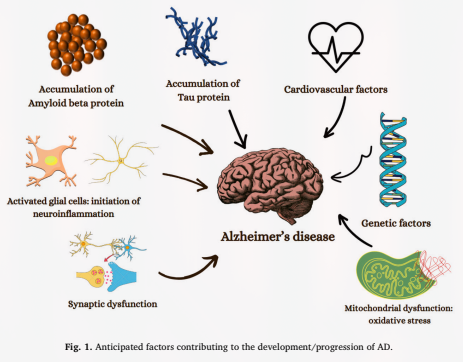
\includegraphics[width=0.6\textwidth]{img/ad_diagram_of_factors.png}
        \caption{caption}
        \label{fig:label}
    \end{figure}
\end{frame}


\begin{frame}{References}
\printbibliography
\end{frame}

\begin{frame}{Acknowledgments}
    \begin{block}{}
        \begin{center}
            This work was supported primarily by the National Science Foundation EPSCoR Program under NSF Award OIA-2242812.
        \end{center}
    \end{block}
\end{frame}

\begin{frame}{Closing}
    \begin{block}{}
       \centering Thank you. Questions?
    \end{block}
\end{frame}

\end{document}
